\chapter{Data Ingestion}

When it comes to using data coming from one or more sources, being them sensors or user activities from a website, there needs to be adequate tools for handling, gathering and routing them inside the cluster where they will be processed.

\section{Kafka}

\textbf{\href{https://kafka.apache.org}{Apache Kafka}} \cite{kafka_doc} is a distributed streaming platform which allows publishing and subscription to streams of records, similarly to a message queue or messaging systems, while storing those streams in a fault-tolerant way and optionally processing them as soon as they enter the system. 

It is mainly used for building real-time streaming data pipelines that need to reliably get data between systems or applications, but also when real-time streaming applications need to transform or react to the streams of data.

Kafka is run on one or more servers as a cluster, storing streams of \textit{records} in categories called \textit{topics}. Each record consists of a key, a value and a timestamp.

It has two main core APIs, \textbf{Producer and Consumer API}, the basic blocks to create streams, but it's possible to use two more sets of APIs: the \textbf{Streams API}, which can be used to process the records and transform them between two or more topics, and the \textbf{Connect API}, which allows to run producers and consumers that connect to other applications or data systems.

\subsection{Topics}

A topic is a category or feed name where records are published. Topics in Kafka are always multi-subscriber, since a topic can exist regardless of the actual consuming of its records, with zero, one, or many consumers that subscribe to the data written to it.

For each topic, the Kafka cluster maintains a partitioned log, where each partition is an ordered, immutable sequence of records that is continually appended to. A sequential id number called \textit{offset} is assigned to each record within a partition as a unique identifier.

The Kafka cluster, through a configurable retention period, retains all published records, whether or not they have been consumed, so that if, for example, the retention policy is set to three days, then a published record is available for consumption for the following three days, after which it will be discarded to free up space. Taking this into consideration, Kafka's performance is constant with respect to the size of the data stored, causing no actual concern if data need to be stored for a long time.


\begin{figure}[h]
    \centering
    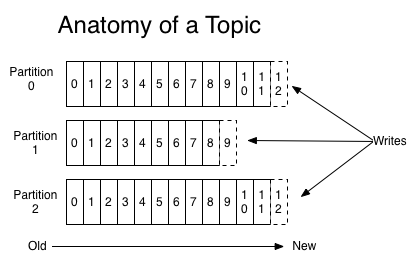
\includegraphics[width=0.7\linewidth]{Figures/log_anatomy}
    \caption[How partition works in a kafka topic]{How partitioning works in a kafka topic. Source: \cite{kafka_doc}}
    \label{fig:loganatomy}
\end{figure}

Only the offset or position of a consumer is retained as metadata, on a per-consumer basis. This offset is completely controllable by the consumer, so that if normally it would advance linearly, the consumer could consume records in any possible order. For example, a consumer can reset to an older offset or, conversely, skip ahead to consume data from the latest record, according to its own policy.

The partitions in the log allow for scaling beyond a size that could fit on a single server, since a topic can handle an arbitrary amount of data, but each individual partition must fit on the servers that host it, and act as the unit of parallelism, so that it's possible to increase the number of partitions of a topic as needed, according to the required throughput.

\subsection{Producers and Consumers}

\paragraph{Producers} They are the components that publish the data to the topics of their choice. They handle the assignment of each record to the partitions within the topic. This is usually done according to a round-robin scheduling, to favour balance loading, or otherwise with a semantic partition function (such as it may be the key of a record).

\paragraph{Consumers} They are labelled with a \textit{consumer group} name, and each record published to a topic is consumed by one consuming instance within each subscribing consumer group. Each instance can be in separate processes or even on separate machines.

A common configuration has topics with a small number of consumer groups, one for each "logical subscriber", where each group, for scalability and fault tolerance purposes, is composed of many consumer instances.

\begin{figure}[h]
    \centering
    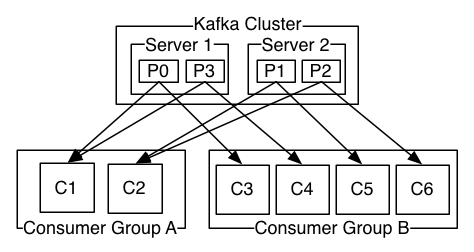
\includegraphics[width=0.7\linewidth]{Figures/consumer-groups}
    \caption[Consumer groups subscribing to a Kafka Cluster]{Consumer groups subscribing to a Kafka Cluster. Source: \cite{kafka_doc}}
    \label{fig:consumer-groups}
\end{figure}


The way Kafka implements consumption is by dividing up the partitions in the log over the consumer instances so that each instance gets a "fair share" of partitions reserved at any point in time. If new instances join the group, Kafka will handle dynamically this addition by giving away some partitions from other members of the group, in order to preserve the fair sharing. Otherwise, if an instance dies, its partitions will be distributed to the remaining instances.

A total order over records is provided only within a partition, and not between different partitions in a topic. However, if a total order over records within a topic is required, than a single partition is needed, consequently meaning that there can only be one consumer process per consumer group. 

\subsection{Use cases}

\paragraph{Messaging}

Kafka can be used as a replacement for a more traditional message broker, for reasons such as decoupling processing from data producers and buffering unprocessed messages. In comparison to most messaging systems, Kafka provides replication, better throughput, built-in partitioning and fault-tolerance, being then a very good solution for large scale message processing applications.

In this domain, Kafka can be compared to  \href{https://www.rabbitmq.com/}{RabbitMQ} and \href{http://activemq.apache.org/}{ActiveMQ}, two of most used traditional messaging systems.

\paragraph{Log Aggregation}

Log aggregation usually collects log files off servers and puts them in a central place, such as a file server or HDFS, for processing purposes. Kafka gives a cleaner abstraction of log or event data as a stream of messages, abstracting away the details of files and allowing, in addition, for lower-latency processing and easier support for multiple data sources and distributed data consumption. In comparison to log-centric systems like Flume, Kafka offers a much lower end-to-end latency and stronger durability guarantees due to replication, while providing equally good performances. 
 
\paragraph{Activity Tracking \& Metrics}

The original use case for Kafka was to rebuild a user activity tracking pipeline as a set of real-time publish-subscribe feeds. Thus decomposing site activity, such as page views, searches, or other actions users may take, publishing records to one topic per activity type. These feeds would be available to subscription for real-time processing or monitoring, and loading into any data warehousing system for offline processing and reporting.

Kafka is often used for aggregating statistics from distributed applications in order to produce centralized feeds for operational monitoring purposes, providing a fault-tolerant monitoring pipeline with low latency.


\section{NiFi}

\textbf{Apache NiFi} \cite{nifi_doc} is a distributed system for centralising, processing and distributing streams of data across a cluster. Its main feature is a web GUI allowing to visually structure the data flow directly from the sources through the definition of graphs where each vertex is called \textbf{Processor} and each edge in-between is a queue in which the \textbf{Flowfiles}, objects wrapping a single records, wait if the processor is busy.

NiFi allows for the creation of a secure cluster where each node takes care of processing a fraction of the Flowfiles circulating inside the graph, load balancing in case of node failures. 

\subsection{FlowFiles}

A \textbf{FlowFile} represents a single piece of data in NiFi, made up of two components: \textbf{FlowFile Attributes} and \textbf{FlowFile Content}. The FlowFile Content is the actual payload, the data that is represented by the FlowFile, while the attributes are characteristics that provide information or context about that data, consisting of key-value pairs. 

All FlowFiles have the following standard attributes:

\begin{itemize}
    \item \textbf{uuid}: A unique identifier for the FlowFile
    
    \item \textbf{filename}: A human-readable filename that may be used when storing the data to disk or in an external service
    
    \item \textbf{path}: A hierarchically structured value that can be used when storing data to disk or an external service so that the data is not stored in a single directory
\end{itemize}

\subsection{Processors}

As already mentioned a \textbf{Processor} is the basic block for the graph structure of a NiFi flow. There are a great variety of Processors built-in, ranging in function from database connections for insertions or queries and producers and consumers for queue processes such as Kafka, to object manipulation such as JSON or XML splitting and fetching and ingestion from sources like web sockets or filesystems.

A single processor can be scheduled to run periodically or continuously and can be configured with the number of concurrent threads that can be used for the execution. Each Processor has different output ports according to the results of the Flowfile processing: \textit{success}, \textit{failure} or other processor-specific routes (e.g. \textit{\textbf{SplitText}} processor, used to split text according to user-specified rules has \textit{original} and \textit{splits} as additional output ports, used to convey in different routes Flowfiles both before and after being split).